\documentclass[a4paper,10pt]{article}
% Use ctrl + alt + V to view live pdf

% Packages
\usepackage[utf8]{inputenc} % For encoding
\usepackage[T1]{fontenc} % Better handling of accented characters and hyphenation
\usepackage{microtype} % Improves spacing and justification
\usepackage{amsmath, amssymb} % For equations and symbols
\usepackage{graphicx} % For including graphics/images
\usepackage{caption} % For customizing figure and table captions
\usepackage{subcaption} % For subfigures and subcaptions
\usepackage{float} % For fixing figure and table positions
\usepackage{booktabs} % For professional-looking tables
\usepackage{siunitx} % For consistent typesetting of units and numbers
\usepackage[margin=2cm]{geometry} % Adjusts page margins
\usepackage{fancyhdr} % For custom headers and footers
\usepackage{lmodern} % For a professional-looking font (main body font)
\usepackage{titlesec} % For title customization
\usepackage{array} % For custom table formatting
\usepackage[colorlinks=true, linkcolor=black, urlcolor=black]{hyperref} % Colored links without boxes
\usepackage{cleveref} % For improved cross-referencing    
\usepackage{multirow}
\usepackage{enumitem}
\usepackage{listings}
\usepackage{xcolor}
\usepackage{textcomp}
\usepackage{tabularx}
\usepackage{changepage}
\usepackage{tikz}
\usepackage{pdfpages}
\usetikzlibrary{shapes.geometric, arrows}
\newcolumntype{Y}{>{\centering\arraybackslash}X}


\lstdefinestyle{vhdl-style}{
    language=VHDL,
    basicstyle=\ttfamily\footnotesize,
    keywordstyle=\bfseries\color{blue},
    commentstyle=\itshape\color{gray},
    stringstyle=\color{red},
    numbers=left,
    numberstyle=\tiny\color{gray},
    stepnumber=1,
    breaklines=true,
    showstringspaces=false,
    frame=single
}
\lstset{style=vhdl-style}
\lstset{captionpos=b}
\lstset{basicstyle=\ttfamily\scriptsize} 
\renewcommand{\lstlistingname}{Program}

% Custom settings
\pagestyle{fancy}
\fancyhf{}
\fancyhead[L]{\textit{GB3 - Risc-V Processor}} % Header left
\fancyhead[R]{\textit{Will Hewes - wh365}} % Header right 
\fancyfoot[C]{\thepage} % Footer center
\setlength{\headheight}{15pt} % Header height
\setlength{\parindent}{0em} % Indentation for paragraphs
\setlength{\parskip}{0.2em} % Add spacing between paragraphs
\setlength{\abovedisplayskip}{0.5em}
\setlength{\belowdisplayskip}{0.5em}
\setlength{\abovedisplayshortskip}{0.5em}
\setlength{\belowdisplayshortskip}{0.5em}
% \setlist{topsep=0em, partopsep=0em, itemsep=0em, parsep=0em}

\graphicspath{{Images/}}

% \renewcommand{\arraystretch}{1.2}

% Title formatting
\renewcommand{\maketitle}{
    \begin{center}
        \LARGE \textbf{ENGINEERING TRIPOS PART IIA} \\ 
        \vspace{0.5em}
        \Large \textbf{GB3 - Risc-V Processor} \\ 
        \vspace{0.5em}
        \textbf{Second Interim Report} \\
        \large Group 4 - Resource Usage \\
        \vspace{1em}
        \large Will Hewes - wh365 \\ 
        Pembroke College \\ 
        \vspace{0.5em}
    \end{center}
}

\begin{document}
%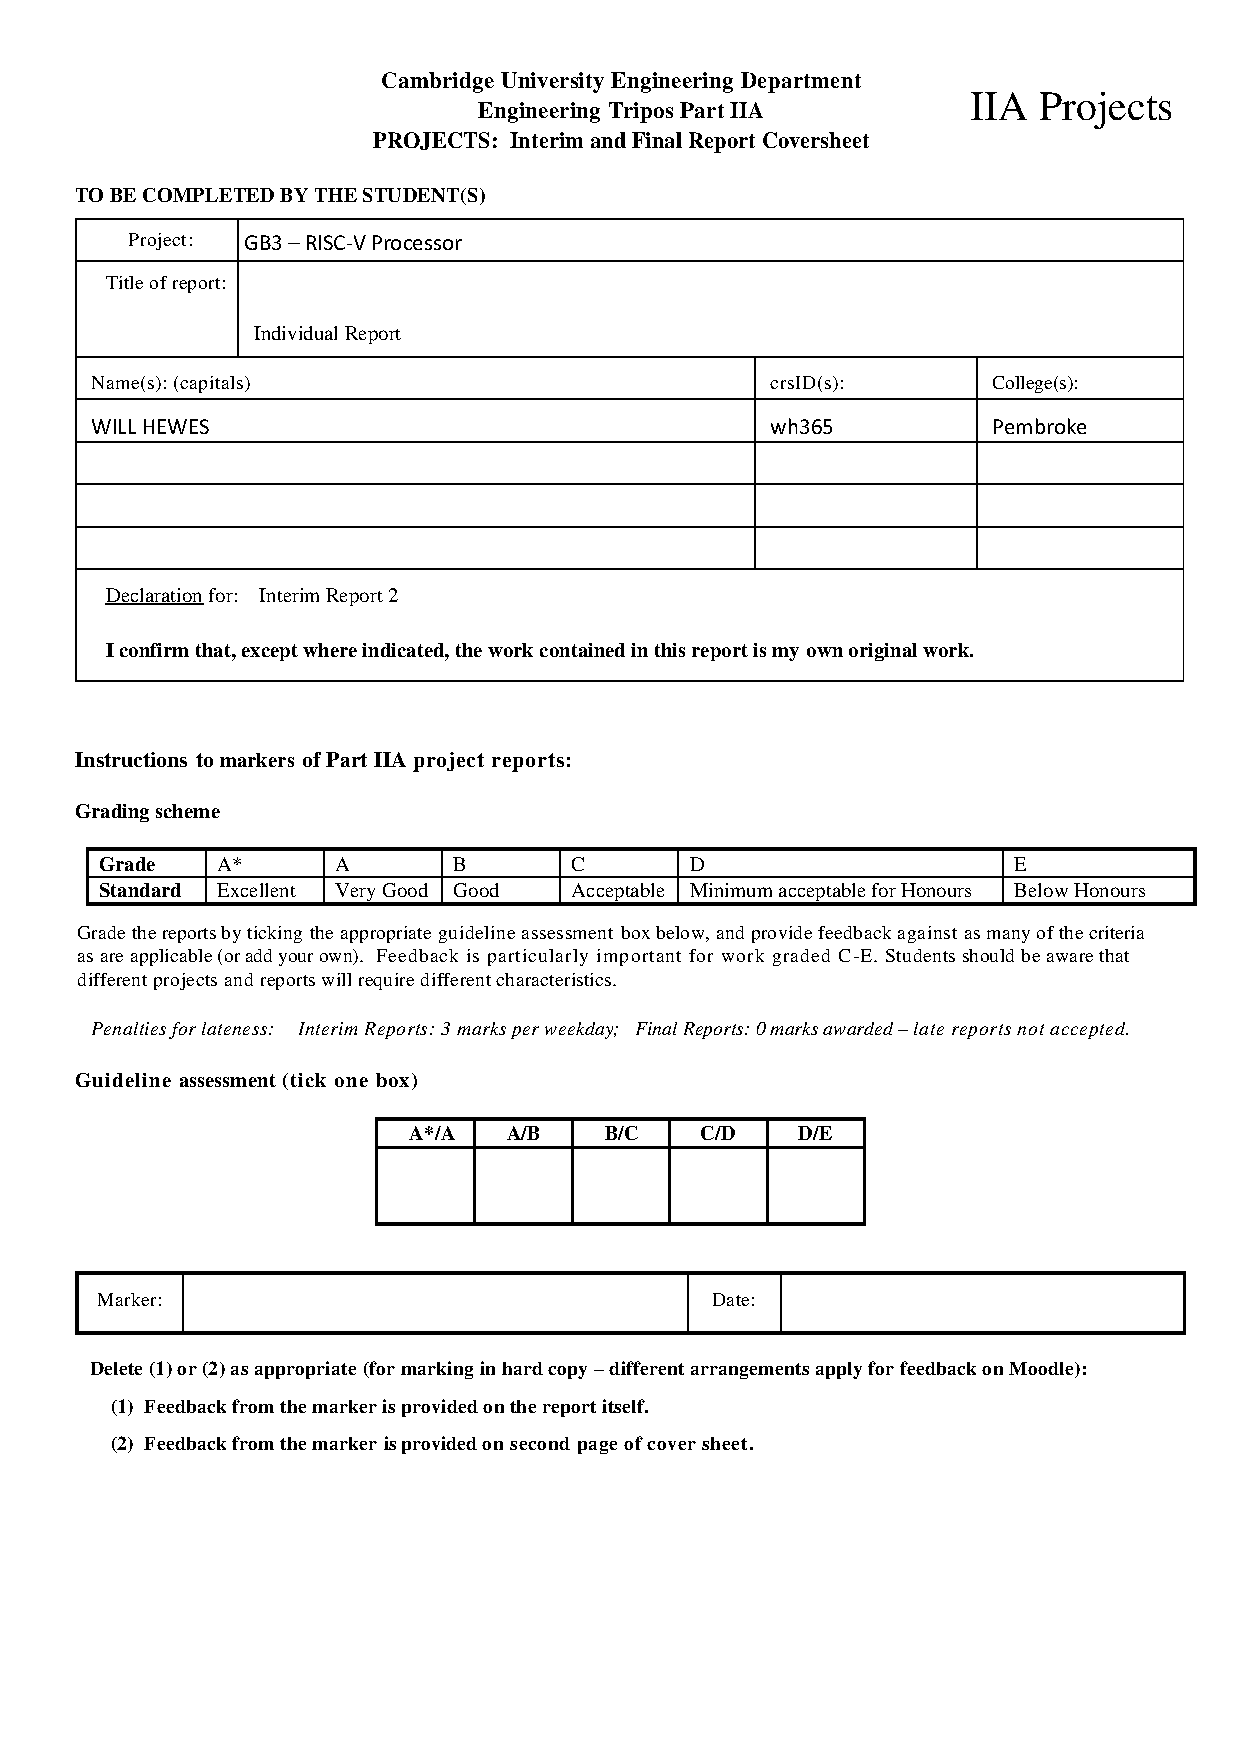
\includepdf[pages=-]{Handouts/IIA Project Coversheet Feedback Interim Report 2.pdf}
\maketitle
\hrule
\tableofcontents
\newpage

\section{Introduction}
\label{sec:Introduction}
% This section should give a detailed introduction to the changes
% you have implemented for your role on the team 
% (power/energy, time, or resource efficiency).

This project involves the collaborative design and implementation 
of a RISC-V processor on an iCE40 FPGA device. 
The overarching aim is to optimise 
the processor design with respect to its 
performance, power dissipation, and resource usage, 
while balancing trade-offs between these three aspects. 
Each team member is responsible for focusing on one of the three aspects.
My reports will focus on the resource usage of the design.

This report outlines the work carried out to reduce resource usage 
in the RISC-V processor implementation. 
My focus has been on optimising the Verilog modules 
most critical to logic utilisation, 
including the adder and program counter clock gating. 
The goal has been to reduce the number of LUTs and flip-flops consumed
by the processor while minimising 
excessive power dissipation or performance degredation.
These modifications form part of a broader group effort targeting performance, 
power consumption, and resource usage. 
Coordination has been ongoing to ensure our changes are compatible and 
contribute towards a coherent final design.

The analysis has primarily been concerning the
\texttt{bubblesort} program due to its increased complexity,
allowing the processor to be pushed further and 
offering more representative resource utilisation patterns.
Preliminary synthesis results indicated that the original design 
made no use of available DSP blocks, 
instead relying heavily on general-purpose LUTs for arithmetic operations.

\section{Preliminary Results}
\label{sec:Preliminary_Results}
% This section should provide detailed quantitative information and results so far
All tables provided will be in order of the changes that were made
and displayed in the Appendix, alongside relevant code snippets.
\subsection{Baseline}
\label{sec:Baseline}

Having performed the baseline analysis in the previous interim report,
the resource usage for the provided processor on the \texttt{bubblesort}
algorithm is shown in table \ref{tab:baseline} the Appendix.

In the baseline design, 
synthesis of the unmodified processor design showed that approximately 
58\% of the available logic cells on the iCE40 UP5K were in use,
along with two third of the available Block RAMs. 
This figure indicates limited headroom for 
further feature integration or pipeline complexity, 
motivating efforts to streamline key datapaths and control logic. 
In particular, duplication in ALU operations, bloated forwarding logic, 
and excess register usage were identified 
as contributors to excessive logic usage. 
Additionally, the design made no use of the available DSPs,
instead implementing its adder functions through LUTs.
These observations guided the subsequent design changes detailed in this report.

\subsection{Program Counter Clock Gating}
\label{sec:Program_Counter_Clock_Gating}

To reduce unnecessary switching activity in the control path, 
support for gated updates to the program counter was introduced. 
This involved modifying the program\_counter.v module 
to accept a write\_enable signal, 
allowing updates to be conditionally applied 
only when pipeline progression is required. 
The cpu.v module was updated accordingly to assert write\_enable 
whenever the stall signal is low, 
ensuring that the PC is held stable during pipeline stalls.

This change helps avoid logic toggling during idle or stalled cycles. 
This primarily has implications toward the power consumption, 
allowing the board to reduce unnecessary dynamic power dissipation 
caused by repeated switching in the program counter logic during pipeline stalls. 
The resource utilisation can be seen in 
table \ref{tab:Program_Counter} in the Appendix,
helping free up 9 logic cells.
Although the impact on LUT usage is minimal, 
this is part of a broader strategy to reduce switching 
by selectively enabling pipeline register updates — 
aligning with the power and resource optimisation goals of the project.

\subsection{Removal of CSR Logic}
\label{sec:CSR}

One of the most significant changes made was the complete removal of the 
Control and Status Register (CSR) logic. 
Control and Status Registers are optional RISC-V components used to 
support operating system-level functionality such as 
interrupt handling, timer access, and machine state tracking.

In the baseline design, CSR handling required dedicated decode paths, 
register file access logic, and a separate CSR register file backed by block RAM. 
As CSR instructions were not required for functional correctness in \texttt{bubblesort}, 
this functionality was deemed expendable for the purposes of resource optimisation.
Since the benchmark programs execute purely in machine mode without 
requiring interrupts, exceptions, or privileged features, 
no CSR-related functionality is invoked, 
and their removal does not affect functional correctness.

The removal involved disabling CSR detection in the control unit, 
replacing related wires with fixed constants, and removing the csr\_file module 
and associated datapath multiplexers. 
Registers previously driven by CSR outputs were redirected to bypass logic 
or default values, ensuring that the pipeline remained functionally complete 
without CSR support.

This change resulted in a notable reduction in logic complexity and 
created a marked drop in block RAM usage. 
As seen in table \ref{tab:CSR} in the Appendix,
the logic cell usage dropped from 3064 to 2905, 
and the RAM usage dropped from 20 to 12,
freeing up an additional 20\% of the available block RAM.
It also simplifies the decode and 
execution stages, reducing combinational logic depth. 
However, it does remove support for future system-level extensions 
that rely on CSR functionality, and would need to be revisited if 
such features are later required.

\subsection{Unused Control Signal Width}
\label{sec:Signal_Width}

During inspection of the decode and execute stages, 
it was identified that the control signal wire cont\_mux\_out 
was defined as a 32-bit bus, despite only 11 bits being used downstream. 
To simplify the design and reduce unnecessary routing, 
the width was reduced to match actual usage, 
and the custom mux2to1\_11bit module was removed in favour of the standard mux2to1.

This change eliminates unused signal bits, 
improving signal clarity and slightly reducing synthesis complexity. 
As seen in Table \ref{tab:Signal_Width} in the Appendix,
the logic cell usage dropped from 2905 to 2891.
This contributes to improved maintainability 
and more efficient use of the FPGA's routing resources. 
Removing unused logic also helps the synthesiser 
more aggressively optimise signal propagation and packing.
This change is relatively small, but it highlights how careful inspection 
of signal widths and register usage can help reduce bloated or unnecessary logic. 
Although the immediate savings are minor, 
it demonstrates a valuable approach to 
improving routing efficiency and reducing synthesis overhead. 
However, identifying these opportunities can be time-consuming, 
as it requires manually tracing signal usage across modules and pipeline stages.

\section{Potential Risks}
\label{sec:Potential_Risks}
% This section should outline any challenges you ran into, 
% potential risks you see going into the final week, 
% and any steps you are taking to mitigate those risks.

While the changes implemented so far have improved logic utilisation 
without degrading performance significantly, several risks remain that could impact 
the stability or scalability of the processor design.

Firstly, although the use of DSP blocks in the ALU has significantly 
reduced LUT usage, it introduces reliance on fixed hardware resources 
that may become a bottleneck if additional DSP-mapped features are introduced. 
Any further overuse of these blocks could limit parallelism or 
necessitate costly logic workarounds. 
As the original design made use of no DSPs,
it is reasonable to perform this shift.

The most signicant change to the implementation was the removal of CSR logic.
Though this has a very positive impact on the LUT usage and in particular
on the reduction of block RAMs required in the design,
it has implications with regard to 
future extensibility and system-level compatibility. 
By removing CSR support, the processor is no longer capable of handling traps, 
exceptions, or privileged control, which limits its applicability 
in more complex applications such as real-time systems, operating systems, 
or embedded environments requiring timer interrupts or performance monitoring. 
Reintroducing CSR functionality in later stages would likely involve 
re-adding significant logic and memory overhead, 
potentially offsetting the current resource savings.

Lastly, clock gating introduced in the pipeline registers assumes 
correct stalling logic. If the stall signal is incorrectly asserted or delayed, 
it could lead to data hazards, register inconsistencies, or pipeline deadlock. 
This risk increases as the pipeline control logic becomes more intricate.

Continued validation through simulation and synthesis will be necessary 
to ensure that further optimisation efforts do not compromise correctness 
or long-term maintainability.

\section{Future Work}
\label{sec:Future_Work}

\section{Conclusion}
\label{sec:Conclusion}

\newpage
\appendix
%Use this section to include diagrams, Verilog or C code, etc
\section{Resource Usage Data}

\begin{table}[H] 
    \centering
    \begin{tabularx}{0.6\textwidth}{X c c}
        \toprule
        Resource type & Used & \% of total \\ \midrule
        Logic cells (\texttt{ICESTORM\_LC}) & 3073 / 5280 & 58\,\% \\
        Block RAMs (\texttt{ICESTORM\_RAM}) & 20 / 30 & 66\,\% \\
        IO buffers (\texttt{SB\_IO}) & 8 / 96 & 8\,\% \\
        Global buffers (\texttt{SB\_GB}) & 5 / 8 & 62\,\% \\
        HF oscillators (\texttt{ICESTORM\_HFOSC}) & 1 / 1 & 100\,\% \\
        \bottomrule
    \end{tabularx}
    \caption{Baseline report}
    \label{tab:baseline}
\end{table}

\begin{table}[H] 
    \centering
    \begin{tabularx}{0.6\textwidth}{X c c}
        \toprule
        Resource type & Used & \% of total \\ \midrule
        Logic cells (\texttt{ICESTORM\_LC}) & 3064 / 5280 & 57\,\% \\
        Block RAMs (\texttt{ICESTORM\_RAM}) & 20 / 30 & 66\,\% \\
        IO buffers (\texttt{SB\_IO}) & 8 / 96 & 8\,\% \\
        Global buffers (\texttt{SB\_GB}) & 5 / 8 & 62\,\% \\
        HF oscillators (\texttt{ICESTORM\_HFOSC}) & 1 / 1 & 100\,\% \\
        \bottomrule
    \end{tabularx}
    \caption{Report after adding clock gating to the Program Counter module}
    \label{tab:Program_Counter}
\end{table}

\begin{table}[H] 
    \centering
    \begin{tabularx}{0.6\textwidth}{X c c}
        \toprule
        Resource type & Used & \% of total \\ \midrule
        Logic cells (\texttt{ICESTORM\_LC}) & 2905 / 5280 & 57\,\% \\
        Block RAMs (\texttt{ICESTORM\_RAM}) & 12 / 30 & 66\,\% \\
        IO buffers (\texttt{SB\_IO}) & 8 / 96 & 8\,\% \\
        Global buffers (\texttt{SB\_GB}) & 5 / 8 & 62\,\% \\
        HF oscillators (\texttt{ICESTORM\_HFOSC}) & 1 / 1 & 100\,\% \\
        \bottomrule
    \end{tabularx}
    \caption{Report after removing Control and Status Register (CSR) logic}
    \label{tab:CSR}
\end{table}

\begin{table}[H] 
    \centering
    \begin{tabularx}{0.6\textwidth}{X c c}
        \toprule
        Resource type & Used & \% of total \\ \midrule
        Logic cells (\texttt{ICESTORM\_LC}) & 2891 / 5280 & 57\,\% \\
        Block RAMs (\texttt{ICESTORM\_RAM}) & 12 / 30 & 66\,\% \\
        IO buffers (\texttt{SB\_IO}) & 8 / 96 & 8\,\% \\
        Global buffers (\texttt{SB\_GB}) & 5 / 8 & 62\,\% \\
        HF oscillators (\texttt{ICESTORM\_HFOSC}) & 1 / 1 & 100\,\% \\
        \bottomrule
    \end{tabularx}
    \caption{Report after removing unused control signal width}
    \label{tab:Signal_Width}
\end{table}

\section{Code}

%\section{Interim Report 1}
%\label{sec:{Interim_Report_1}}
%\includepdf[pages=3-]{Reports/wh365-interim-report-1.pdf}

\end{document}